\documentclass[twoside]{book}

% Packages required by doxygen
\usepackage{fixltx2e}
\usepackage{calc}
\usepackage{doxygen}
\usepackage[export]{adjustbox} % also loads graphicx
\usepackage{graphicx}
\usepackage[utf8]{inputenc}
\usepackage{makeidx}
\usepackage{multicol}
\usepackage{multirow}
\PassOptionsToPackage{warn}{textcomp}
\usepackage{textcomp}
\usepackage[nointegrals]{wasysym}
\usepackage[table]{xcolor}

% Font selection
\usepackage[T1]{fontenc}
\usepackage[scaled=.90]{helvet}
\usepackage{courier}
\usepackage{amssymb}
\usepackage{sectsty}
\renewcommand{\familydefault}{\sfdefault}
\allsectionsfont{%
  \fontseries{bc}\selectfont%
  \color{darkgray}%
}
\renewcommand{\DoxyLabelFont}{%
  \fontseries{bc}\selectfont%
  \color{darkgray}%
}
\newcommand{\+}{\discretionary{\mbox{\scriptsize$\hookleftarrow$}}{}{}}

% Page & text layout
\usepackage{geometry}
\geometry{%
  a4paper,%
  top=2.5cm,%
  bottom=2.5cm,%
  left=2.5cm,%
  right=2.5cm%
}
\tolerance=750
\hfuzz=15pt
\hbadness=750
\setlength{\emergencystretch}{15pt}
\setlength{\parindent}{0cm}
\setlength{\parskip}{0.2cm}
\makeatletter
\renewcommand{\paragraph}{%
  \@startsection{paragraph}{4}{0ex}{-1.0ex}{1.0ex}{%
    \normalfont\normalsize\bfseries\SS@parafont%
  }%
}
\renewcommand{\subparagraph}{%
  \@startsection{subparagraph}{5}{0ex}{-1.0ex}{1.0ex}{%
    \normalfont\normalsize\bfseries\SS@subparafont%
  }%
}
\makeatother

% Headers & footers
\usepackage{fancyhdr}
\pagestyle{fancyplain}
\fancyhead[LE]{\fancyplain{}{\bfseries\thepage}}
\fancyhead[CE]{\fancyplain{}{}}
\fancyhead[RE]{\fancyplain{}{\bfseries\leftmark}}
\fancyhead[LO]{\fancyplain{}{\bfseries\rightmark}}
\fancyhead[CO]{\fancyplain{}{}}
\fancyhead[RO]{\fancyplain{}{\bfseries\thepage}}
\fancyfoot[LE]{\fancyplain{}{}}
\fancyfoot[CE]{\fancyplain{}{}}
\fancyfoot[RE]{\fancyplain{}{\bfseries\scriptsize Generated by Doxygen }}
\fancyfoot[LO]{\fancyplain{}{\bfseries\scriptsize Generated by Doxygen }}
\fancyfoot[CO]{\fancyplain{}{}}
\fancyfoot[RO]{\fancyplain{}{}}
\renewcommand{\footrulewidth}{0.4pt}
\renewcommand{\chaptermark}[1]{%
  \markboth{#1}{}%
}
\renewcommand{\sectionmark}[1]{%
  \markright{\thesection\ #1}%
}

% Indices & bibliography
\usepackage{natbib}
\usepackage[titles]{tocloft}
\setcounter{tocdepth}{3}
\setcounter{secnumdepth}{5}
\makeindex

% Hyperlinks (required, but should be loaded last)
\usepackage{ifpdf}
\ifpdf
  \usepackage[pdftex,pagebackref=true]{hyperref}
\else
  \usepackage[ps2pdf,pagebackref=true]{hyperref}
\fi
\hypersetup{%
  colorlinks=true,%
  linkcolor=blue,%
  citecolor=blue,%
  unicode%
}

% Custom commands
\newcommand{\clearemptydoublepage}{%
  \newpage{\pagestyle{empty}\cleardoublepage}%
}

\usepackage{caption}
\captionsetup{labelsep=space,justification=centering,font={bf},singlelinecheck=off,skip=4pt,position=top}

%===== C O N T E N T S =====

\begin{document}

% Titlepage & ToC
\hypersetup{pageanchor=false,
             bookmarksnumbered=true,
             pdfencoding=unicode
            }
\pagenumbering{roman}
\begin{titlepage}
\vspace*{7cm}
\begin{center}%
{\Large My Project }\\
\vspace*{1cm}
{\large Generated by Doxygen 1.8.11}\\
\end{center}
\end{titlepage}
\clearemptydoublepage
\tableofcontents
\clearemptydoublepage
\pagenumbering{arabic}
\hypersetup{pageanchor=true}

%--- Begin generated contents ---
\chapter{Namespace Index}
\section{Namespace List}
Here is a list of all documented namespaces with brief descriptions\+:\begin{DoxyCompactList}
\item\contentsline{section}{\hyperlink{namespaceblocks}{blocks} \\*Class file for the blocks }{\pageref{namespaceblocks}}{}
\item\contentsline{section}{\hyperlink{namespaceplayer}{player} \\*Defined the behaviors of the player }{\pageref{namespaceplayer}}{}
\end{DoxyCompactList}

\chapter{Hierarchical Index}
\section{Class Hierarchy}
This inheritance list is sorted roughly, but not completely, alphabetically\+:\begin{DoxyCompactList}
\item object\begin{DoxyCompactList}
\item \contentsline{section}{main\+Game\+Loop.\+Camera}{\pageref{classmain_game_loop_1_1_camera}}{}
\item \contentsline{section}{pyganim.\+Pyg\+Animation}{\pageref{classpyganim_1_1_pyg_animation}}{}
\item \contentsline{section}{pyganim.\+Pyg\+Conductor}{\pageref{classpyganim_1_1_pyg_conductor}}{}
\end{DoxyCompactList}
\item Sprite\begin{DoxyCompactList}
\item \contentsline{section}{blocks.\+Platform}{\pageref{classblocks_1_1_platform}}{}
\begin{DoxyCompactList}
\item \contentsline{section}{blocks.\+Block\+Die}{\pageref{classblocks_1_1_block_die}}{}
\item \contentsline{section}{blocks.\+Princess}{\pageref{classblocks_1_1_princess}}{}
\end{DoxyCompactList}
\item \contentsline{section}{monsters.\+Monster}{\pageref{classmonsters_1_1_monster}}{}
\item \contentsline{section}{player.\+Player}{\pageref{classplayer_1_1_player}}{}
\end{DoxyCompactList}
\end{DoxyCompactList}

\chapter{Class Index}
\section{Class List}
Here are the classes, structs, unions and interfaces with brief descriptions\+:\begin{DoxyCompactList}
\item\contentsline{section}{\hyperlink{classblocks_1_1_block_die}{blocks.\+Block\+Die} \\*Blocks that would kill the player }{\pageref{classblocks_1_1_block_die}}{}
\item\contentsline{section}{\hyperlink{classmain_game_loop_1_1_camera}{main\+Game\+Loop.\+Camera} \\*Class for the camera }{\pageref{classmain_game_loop_1_1_camera}}{}
\item\contentsline{section}{\hyperlink{classmonsters_1_1_monster}{monsters.\+Monster} \\*\hyperlink{classmonsters_1_1_monster}{Monster} class using pygame.\+sprite }{\pageref{classmonsters_1_1_monster}}{}
\item\contentsline{section}{\hyperlink{classblocks_1_1_platform}{blocks.\+Platform} \\*Blocks that makes the platform }{\pageref{classblocks_1_1_platform}}{}
\item\contentsline{section}{\hyperlink{classplayer_1_1_player}{player.\+Player} \\*\hyperlink{classplayer_1_1_player}{Player} class }{\pageref{classplayer_1_1_player}}{}
\item\contentsline{section}{\hyperlink{classblocks_1_1_princess}{blocks.\+Princess} \\*The end of the game }{\pageref{classblocks_1_1_princess}}{}
\item\contentsline{section}{\hyperlink{classpyganim_1_1_pyg_animation}{pyganim.\+Pyg\+Animation} }{\pageref{classpyganim_1_1_pyg_animation}}{}
\item\contentsline{section}{\hyperlink{classpyganim_1_1_pyg_conductor}{pyganim.\+Pyg\+Conductor} }{\pageref{classpyganim_1_1_pyg_conductor}}{}
\end{DoxyCompactList}

\chapter{Namespace Documentation}
\hypertarget{namespaceblocks}{}\section{blocks Namespace Reference}
\label{namespaceblocks}\index{blocks@{blocks}}


class file for the blocks  


\subsection*{Classes}
\begin{DoxyCompactItemize}
\item 
class \hyperlink{classblocks_1_1_block_die}{Block\+Die}
\begin{DoxyCompactList}\small\item\em blocks that would kill the player \end{DoxyCompactList}\item 
class \hyperlink{classblocks_1_1_platform}{Platform}
\begin{DoxyCompactList}\small\item\em blocks that makes the platform \end{DoxyCompactList}\item 
class \hyperlink{classblocks_1_1_princess}{Princess}
\begin{DoxyCompactList}\small\item\em The end of the game. \end{DoxyCompactList}\end{DoxyCompactItemize}
\subsection*{Variables}
\begin{DoxyCompactItemize}
\end{DoxyCompactItemize}


\subsection{Detailed Description}
class file for the blocks 
\hypertarget{namespacemain}{}\section{main Namespace Reference}
\label{namespacemain}\index{main@{main}}


this is the main file for our game  




\subsection{Detailed Description}
this is the main file for our game 
\hypertarget{namespacemonsters}{}\section{monsters Namespace Reference}
\label{namespacemonsters}\index{monsters@{monsters}}


class file for monster  


\subsection*{Classes}
\begin{DoxyCompactItemize}
\item 
class \hyperlink{classmonsters_1_1_monster}{Monster}
\begin{DoxyCompactList}\small\item\em monster class using pygame.\+sprite \end{DoxyCompactList}\end{DoxyCompactItemize}
\subsection*{Variables}
\begin{DoxyCompactItemize}
\end{DoxyCompactItemize}


\subsection{Detailed Description}
class file for monster 
\hypertarget{namespaceplayer}{}\section{player Namespace Reference}
\label{namespaceplayer}\index{player@{player}}


Defined the behaviors of the player.  


\subsection*{Classes}
\begin{DoxyCompactItemize}
\item 
class \hyperlink{classplayer_1_1_player}{Player}
\begin{DoxyCompactList}\small\item\em \hyperlink{classplayer_1_1_player}{Player} class. \end{DoxyCompactList}\end{DoxyCompactItemize}
\subsection*{Variables}
\begin{DoxyCompactItemize}
\end{DoxyCompactItemize}


\subsection{Detailed Description}
Defined the behaviors of the player. 

\subsection{Variable Documentation}
\index{player@{player}!A\+N\+I\+M\+A\+T\+I\+O\+N\+\_\+\+L\+E\+FT@{A\+N\+I\+M\+A\+T\+I\+O\+N\+\_\+\+L\+E\+FT}}
\index{A\+N\+I\+M\+A\+T\+I\+O\+N\+\_\+\+L\+E\+FT@{A\+N\+I\+M\+A\+T\+I\+O\+N\+\_\+\+L\+E\+FT}!player@{player}}
\subsubsection[{\texorpdfstring{A\+N\+I\+M\+A\+T\+I\+O\+N\+\_\+\+L\+E\+FT}{ANIMATION_LEFT}}]{\setlength{\rightskip}{0pt plus 5cm}list player.\+A\+N\+I\+M\+A\+T\+I\+O\+N\+\_\+\+L\+E\+FT}\hypertarget{namespaceplayer_ae86d8b914785e2c3229383c956d87836}{}\label{namespaceplayer_ae86d8b914785e2c3229383c956d87836}
{\bfseries Initial value\+:}
\begin{DoxyCode}
1 = [(\textcolor{stringliteral}{'%s/mario/l1.png'}% ICON\_DIR), 
2             (\textcolor{stringliteral}{'%s/mario/l2.png'}% ICON\_DIR), 
3             (\textcolor{stringliteral}{'%s/mario/l3.png'}% ICON\_DIR), 
4             (\textcolor{stringliteral}{'%s/mario/l4.png'}% ICON\_DIR), 
5             (\textcolor{stringliteral}{'%s/mario/l5.png'}% ICON\_DIR)]
\end{DoxyCode}
\index{player@{player}!A\+N\+I\+M\+A\+T\+I\+O\+N\+\_\+\+R\+I\+G\+HT@{A\+N\+I\+M\+A\+T\+I\+O\+N\+\_\+\+R\+I\+G\+HT}}
\index{A\+N\+I\+M\+A\+T\+I\+O\+N\+\_\+\+R\+I\+G\+HT@{A\+N\+I\+M\+A\+T\+I\+O\+N\+\_\+\+R\+I\+G\+HT}!player@{player}}
\subsubsection[{\texorpdfstring{A\+N\+I\+M\+A\+T\+I\+O\+N\+\_\+\+R\+I\+G\+HT}{ANIMATION_RIGHT}}]{\setlength{\rightskip}{0pt plus 5cm}list player.\+A\+N\+I\+M\+A\+T\+I\+O\+N\+\_\+\+R\+I\+G\+HT}\hypertarget{namespaceplayer_a7ae2af21157d4891b7606e81147b1fa9}{}\label{namespaceplayer_a7ae2af21157d4891b7606e81147b1fa9}
{\bfseries Initial value\+:}
\begin{DoxyCode}
1 = [(\textcolor{stringliteral}{'%s/mario/r1.png'}% ICON\_DIR), 
2             (\textcolor{stringliteral}{'%s/mario/r2.png'}% ICON\_DIR), 
3             (\textcolor{stringliteral}{'%s/mario/r3.png'}% ICON\_DIR), 
4             (\textcolor{stringliteral}{'%s/mario/r4.png'}% ICON\_DIR), 
5             (\textcolor{stringliteral}{'%s/mario/r5.png'}% ICON\_DIR)]
\end{DoxyCode}

\chapter{Class Documentation}
\hypertarget{classblocks_1_1_block_die}{}\section{blocks.\+Block\+Die Class Reference}
\label{classblocks_1_1_block_die}\index{blocks.\+Block\+Die@{blocks.\+Block\+Die}}


blocks that would kill the player  


Inheritance diagram for blocks.\+Block\+Die\+:\begin{figure}[H]
\begin{center}
\leavevmode
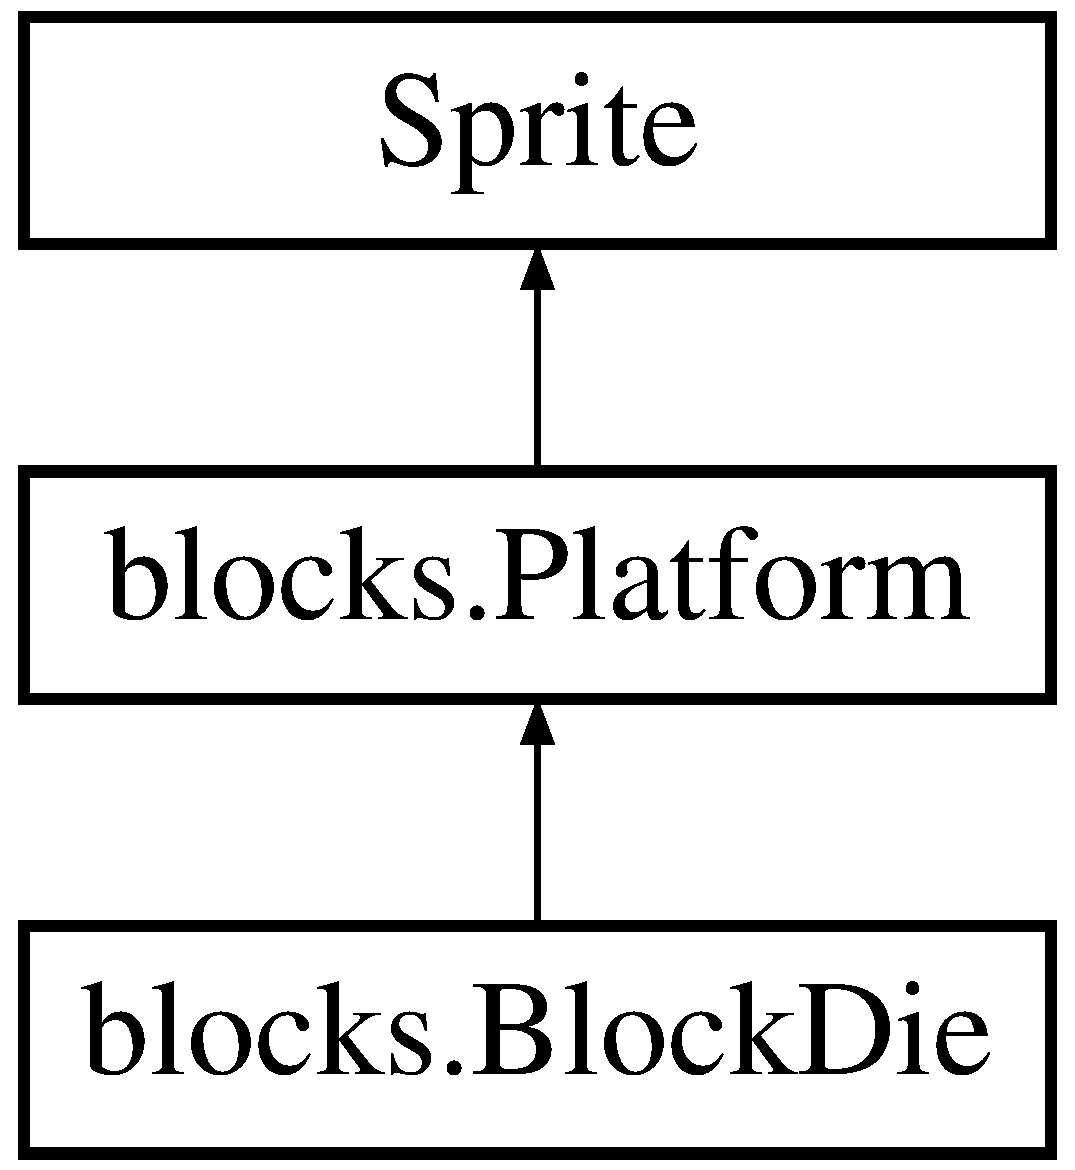
\includegraphics[height=3.000000cm]{classblocks_1_1_block_die}
\end{center}
\end{figure}
\subsection*{Public Member Functions}
\begin{DoxyCompactItemize}
\item 
def \hyperlink{classblocks_1_1_block_die_a993ad71b0a3f9ddb84cb092dd4d0b460}{\+\_\+\+\_\+init\+\_\+\+\_\+} (self, x, y)
\begin{DoxyCompactList}\small\item\em The constructor. \end{DoxyCompactList}\end{DoxyCompactItemize}
\subsection*{Public Attributes}
\begin{DoxyCompactItemize}
\end{DoxyCompactItemize}


\subsection{Detailed Description}
blocks that would kill the player 

\subsection{Constructor \& Destructor Documentation}
\index{blocks\+::\+Block\+Die@{blocks\+::\+Block\+Die}!\+\_\+\+\_\+init\+\_\+\+\_\+@{\+\_\+\+\_\+init\+\_\+\+\_\+}}
\index{\+\_\+\+\_\+init\+\_\+\+\_\+@{\+\_\+\+\_\+init\+\_\+\+\_\+}!blocks\+::\+Block\+Die@{blocks\+::\+Block\+Die}}
\subsubsection[{\texorpdfstring{\+\_\+\+\_\+init\+\_\+\+\_\+(self, x, y)}{__init__(self, x, y)}}]{\setlength{\rightskip}{0pt plus 5cm}def blocks.\+Block\+Die.\+\_\+\+\_\+init\+\_\+\+\_\+ (
\begin{DoxyParamCaption}
\item[{}]{self, }
\item[{}]{x, }
\item[{}]{y}
\end{DoxyParamCaption}
)}\hypertarget{classblocks_1_1_block_die_a993ad71b0a3f9ddb84cb092dd4d0b460}{}\label{classblocks_1_1_block_die_a993ad71b0a3f9ddb84cb092dd4d0b460}


The constructor. 


\begin{DoxyParams}{Parameters}
{\em self} & the object pointer \\
\hline
{\em x} & the x location \\
\hline
{\em y} & the y location \\
\hline
\end{DoxyParams}


The documentation for this class was generated from the following file\+:\begin{DoxyCompactItemize}
\item 
blocks.\+py\end{DoxyCompactItemize}

\hypertarget{classmain_game_loop_1_1_camera}{}\section{main\+Game\+Loop.\+Camera Class Reference}
\label{classmain_game_loop_1_1_camera}\index{main\+Game\+Loop.\+Camera@{main\+Game\+Loop.\+Camera}}


Class for the camera.  


Inheritance diagram for main\+Game\+Loop.\+Camera\+:\begin{figure}[H]
\begin{center}
\leavevmode
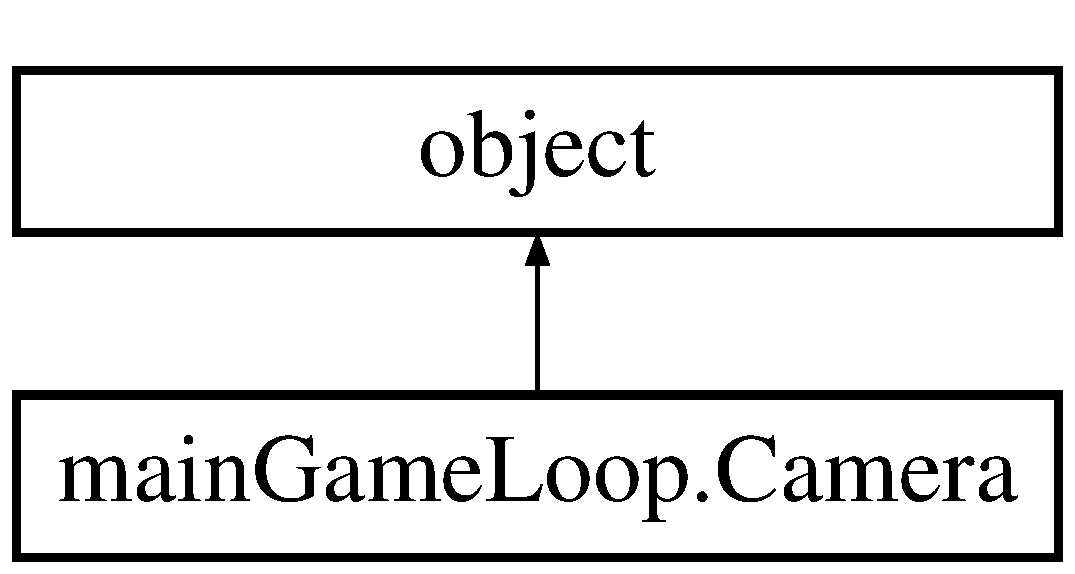
\includegraphics[height=2.000000cm]{classmain_game_loop_1_1_camera}
\end{center}
\end{figure}
\subsection*{Public Member Functions}
\begin{DoxyCompactItemize}
\end{DoxyCompactItemize}
\subsection*{Public Attributes}
\begin{DoxyCompactItemize}
\end{DoxyCompactItemize}


\subsection{Detailed Description}
Class for the camera. 

The documentation for this class was generated from the following file\+:\begin{DoxyCompactItemize}
\item 
main\+Game\+Loop.\+py\end{DoxyCompactItemize}

\hypertarget{classmonsters_1_1_monster}{}\section{monsters.\+Monster Class Reference}
\label{classmonsters_1_1_monster}\index{monsters.\+Monster@{monsters.\+Monster}}
Inheritance diagram for monsters.\+Monster\+:\begin{figure}[H]
\begin{center}
\leavevmode
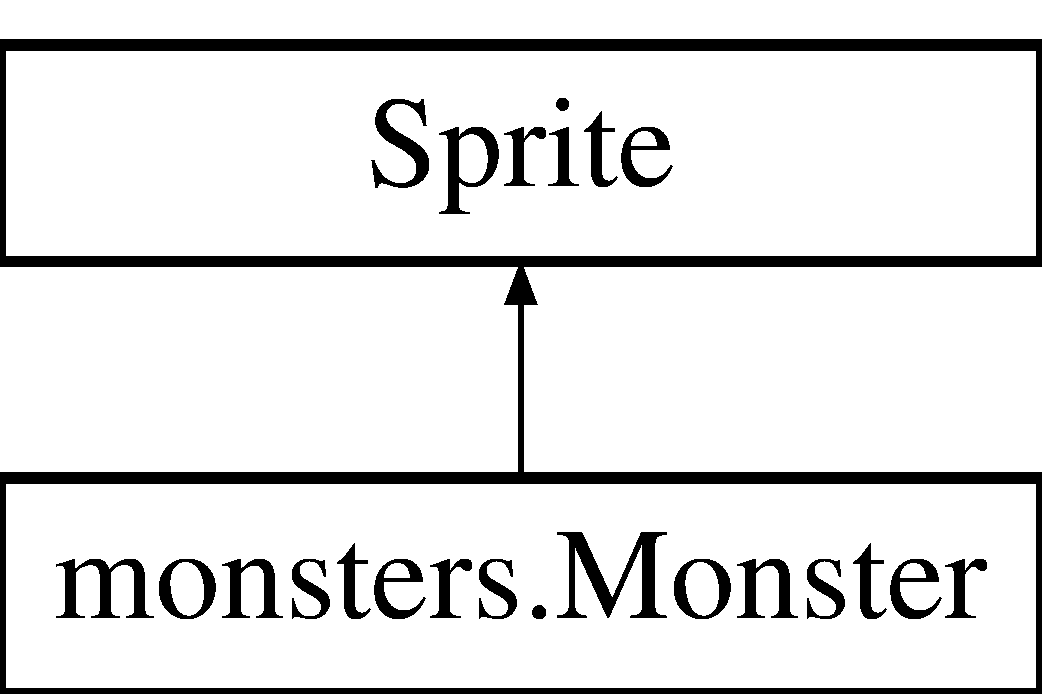
\includegraphics[height=2.000000cm]{classmonsters_1_1_monster}
\end{center}
\end{figure}
\subsection*{Public Member Functions}
\begin{DoxyCompactItemize}
\end{DoxyCompactItemize}
\subsection*{Public Attributes}
\begin{DoxyCompactItemize}
\end{DoxyCompactItemize}


The documentation for this class was generated from the following file\+:\begin{DoxyCompactItemize}
\item 
monsters.\+py\end{DoxyCompactItemize}

\hypertarget{classblocks_1_1_platform}{}\section{blocks.\+Platform Class Reference}
\label{classblocks_1_1_platform}\index{blocks.\+Platform@{blocks.\+Platform}}


blocks that makes the platform  


Inheritance diagram for blocks.\+Platform\+:\begin{figure}[H]
\begin{center}
\leavevmode
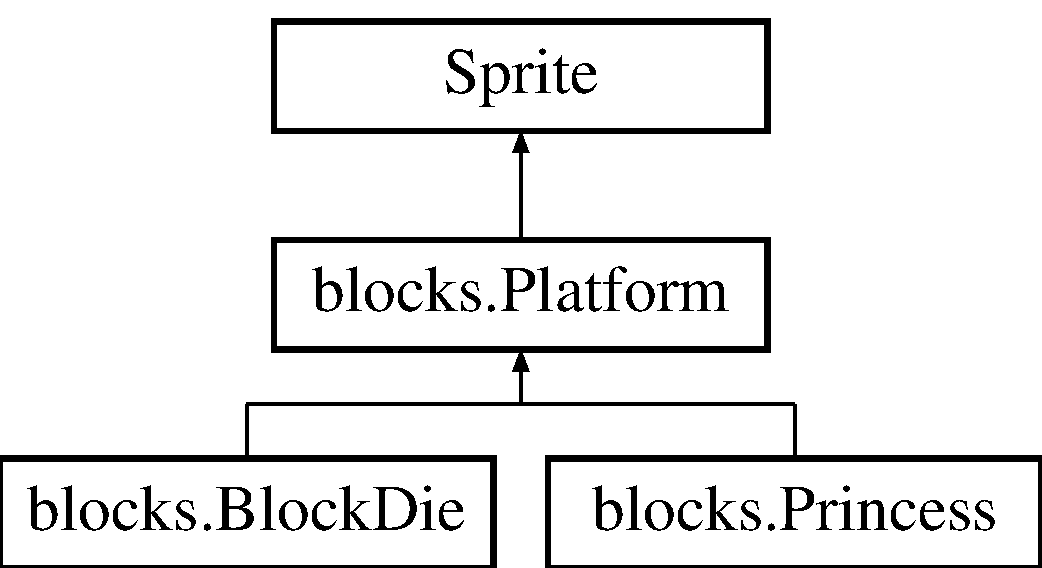
\includegraphics[height=3.000000cm]{classblocks_1_1_platform}
\end{center}
\end{figure}
\subsection*{Public Member Functions}
\begin{DoxyCompactItemize}
\item 
def \hyperlink{classblocks_1_1_platform_a8c0aa810b5e8c4551852e640d99d5c00}{\+\_\+\+\_\+init\+\_\+\+\_\+} (self, x, y)
\begin{DoxyCompactList}\small\item\em The constructor. \end{DoxyCompactList}\end{DoxyCompactItemize}
\subsection*{Public Attributes}
\begin{DoxyCompactItemize}
\end{DoxyCompactItemize}


\subsection{Detailed Description}
blocks that makes the platform 

The basic elements of the game background. 

\subsection{Constructor \& Destructor Documentation}
\index{blocks\+::\+Platform@{blocks\+::\+Platform}!\+\_\+\+\_\+init\+\_\+\+\_\+@{\+\_\+\+\_\+init\+\_\+\+\_\+}}
\index{\+\_\+\+\_\+init\+\_\+\+\_\+@{\+\_\+\+\_\+init\+\_\+\+\_\+}!blocks\+::\+Platform@{blocks\+::\+Platform}}
\subsubsection[{\texorpdfstring{\+\_\+\+\_\+init\+\_\+\+\_\+(self, x, y)}{__init__(self, x, y)}}]{\setlength{\rightskip}{0pt plus 5cm}def blocks.\+Platform.\+\_\+\+\_\+init\+\_\+\+\_\+ (
\begin{DoxyParamCaption}
\item[{}]{self, }
\item[{}]{x, }
\item[{}]{y}
\end{DoxyParamCaption}
)}\hypertarget{classblocks_1_1_platform_a8c0aa810b5e8c4551852e640d99d5c00}{}\label{classblocks_1_1_platform_a8c0aa810b5e8c4551852e640d99d5c00}


The constructor. 


\begin{DoxyParams}{Parameters}
{\em self} & the object pointer \\
\hline
{\em x} & the x location \\
\hline
{\em y} & the y location \\
\hline
\end{DoxyParams}


The documentation for this class was generated from the following file\+:\begin{DoxyCompactItemize}
\item 
blocks.\+py\end{DoxyCompactItemize}

\hypertarget{classplayer_1_1_player}{}\section{player.\+Player Class Reference}
\label{classplayer_1_1_player}\index{player.\+Player@{player.\+Player}}


\hyperlink{classplayer_1_1_player}{Player} class.  


Inheritance diagram for player.\+Player\+:\begin{figure}[H]
\begin{center}
\leavevmode
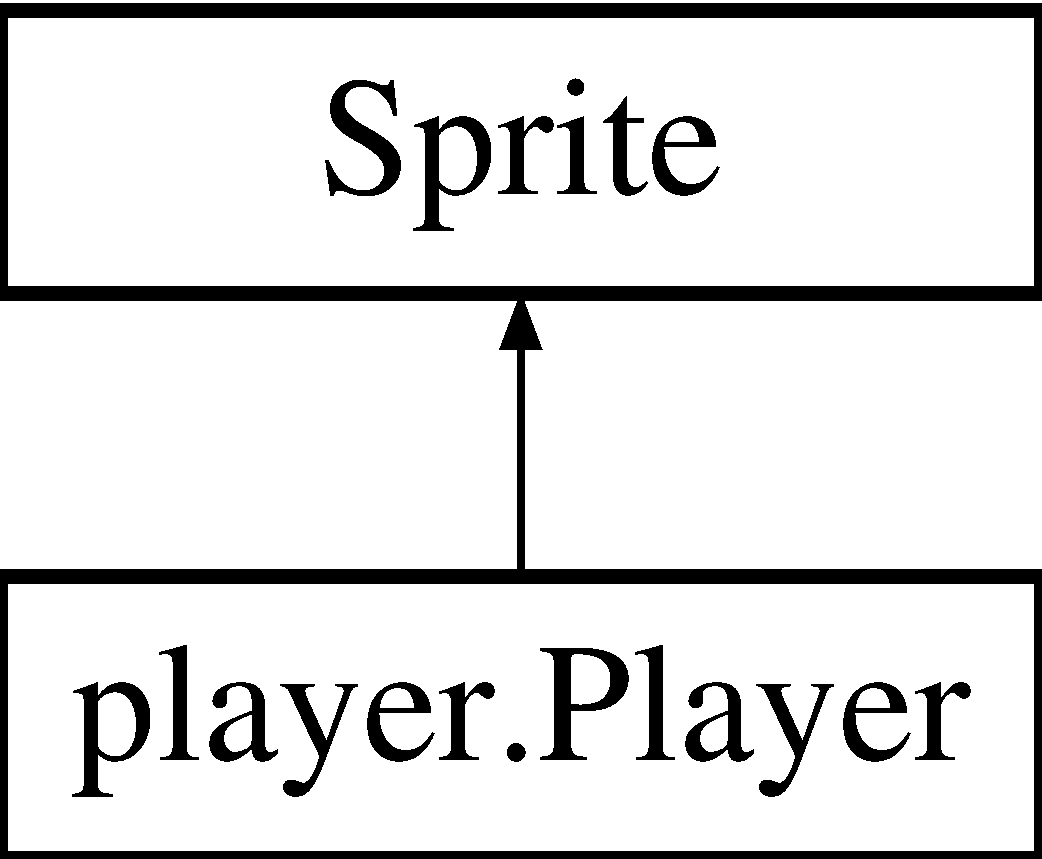
\includegraphics[height=2.000000cm]{classplayer_1_1_player}
\end{center}
\end{figure}
\subsection*{Public Member Functions}
\begin{DoxyCompactItemize}
\item 
def \hyperlink{classplayer_1_1_player_a52434c87f8baf931655ff9811c57f288}{\+\_\+\+\_\+init\+\_\+\+\_\+} (self, x, y)
\begin{DoxyCompactList}\small\item\em The constructor. \end{DoxyCompactList}\item 
def \hyperlink{classplayer_1_1_player_ad2ac60cf460239c12977eda3acc99d0c}{update} (self, left, right, up, platforms)
\begin{DoxyCompactList}\small\item\em The method to update the location of the player. \end{DoxyCompactList}\item 
def \hyperlink{classplayer_1_1_player_aaab39aa7f4e9fbb17207cd584641d7e0}{collide} (self, \hyperlink{classplayer_1_1_player_ae073642fcdedce9559f717e60945e51f}{xvel}, \hyperlink{classplayer_1_1_player_a91226d0b71959f0a35b280c6e2774e2d}{yvel}, platforms)
\begin{DoxyCompactList}\small\item\em The method to detect whether there\textquotesingle{}s a collision. \end{DoxyCompactList}\item 
def \hyperlink{classplayer_1_1_player_a6ad207dfcfeabddc8fb8e59dca09aa8e}{teleporting} (self, goX, goY)
\begin{DoxyCompactList}\small\item\em The method to teleport the player. \end{DoxyCompactList}\item 
def \hyperlink{classplayer_1_1_player_ac230f41f1580c1a884799af9fd199b34}{die} (self)
\begin{DoxyCompactList}\small\item\em The method to kill the player. \end{DoxyCompactList}\end{DoxyCompactItemize}
\subsection*{Public Attributes}
\begin{DoxyCompactItemize}
\item 
\hyperlink{classplayer_1_1_player_aba84dd227f561af4f4dda3880912bf1b}{win}\hypertarget{classplayer_1_1_player_aba84dd227f561af4f4dda3880912bf1b}{}\label{classplayer_1_1_player_aba84dd227f561af4f4dda3880912bf1b}

\begin{DoxyCompactList}\small\item\em to keep track whether the game should end \end{DoxyCompactList}\item 
\hyperlink{classplayer_1_1_player_ae073642fcdedce9559f717e60945e51f}{xvel}\hypertarget{classplayer_1_1_player_ae073642fcdedce9559f717e60945e51f}{}\label{classplayer_1_1_player_ae073642fcdedce9559f717e60945e51f}

\begin{DoxyCompactList}\small\item\em velocity in x direction \end{DoxyCompactList}\item 
\hyperlink{classplayer_1_1_player_a91226d0b71959f0a35b280c6e2774e2d}{yvel}\hypertarget{classplayer_1_1_player_a91226d0b71959f0a35b280c6e2774e2d}{}\label{classplayer_1_1_player_a91226d0b71959f0a35b280c6e2774e2d}

\begin{DoxyCompactList}\small\item\em velocity in y direction \end{DoxyCompactList}\item 
\hyperlink{classplayer_1_1_player_a3ad9f576ec329032c97a04f93ff53f88}{on\+Ground}\hypertarget{classplayer_1_1_player_a3ad9f576ec329032c97a04f93ff53f88}{}\label{classplayer_1_1_player_a3ad9f576ec329032c97a04f93ff53f88}

\begin{DoxyCompactList}\small\item\em to see if the character isn\textquotesingle{}t jumping \end{DoxyCompactList}\item 
\hyperlink{classplayer_1_1_player_a7727dfee393c4814eb2cb7090f2f3788}{startX}\hypertarget{classplayer_1_1_player_a7727dfee393c4814eb2cb7090f2f3788}{}\label{classplayer_1_1_player_a7727dfee393c4814eb2cb7090f2f3788}

\begin{DoxyCompactList}\small\item\em the initial x location \end{DoxyCompactList}\item 
\hyperlink{classplayer_1_1_player_a833a43f5890d48e945e62f7759c7c9f7}{startY}\hypertarget{classplayer_1_1_player_a833a43f5890d48e945e62f7759c7c9f7}{}\label{classplayer_1_1_player_a833a43f5890d48e945e62f7759c7c9f7}

\begin{DoxyCompactList}\small\item\em the initial y location \end{DoxyCompactList}\item 
\hyperlink{classplayer_1_1_player_a51ce2953ea3a60d34f3b21f916d4d122}{death\+Counter}\hypertarget{classplayer_1_1_player_a51ce2953ea3a60d34f3b21f916d4d122}{}\label{classplayer_1_1_player_a51ce2953ea3a60d34f3b21f916d4d122}

\begin{DoxyCompactList}\small\item\em count the death \end{DoxyCompactList}\item 
\hyperlink{classplayer_1_1_player_ac3a2325d576ac612ed8b00f0f61fe55b}{image}\hypertarget{classplayer_1_1_player_ac3a2325d576ac612ed8b00f0f61fe55b}{}\label{classplayer_1_1_player_ac3a2325d576ac612ed8b00f0f61fe55b}

\begin{DoxyCompactList}\small\item\em pygame property, the player\textquotesingle{}s image \end{DoxyCompactList}\item 
\hyperlink{classplayer_1_1_player_a6870facb96e50fe33af1071506c67c69}{rect}
\begin{DoxyCompactList}\small\item\em pygame rectangle of the player. \end{DoxyCompactList}\end{DoxyCompactItemize}


\subsection{Detailed Description}
\hyperlink{classplayer_1_1_player}{Player} class. 

This is the class for player, we define some variables to restrain the behaviors of our character. 

\subsection{Constructor \& Destructor Documentation}
\index{player\+::\+Player@{player\+::\+Player}!\+\_\+\+\_\+init\+\_\+\+\_\+@{\+\_\+\+\_\+init\+\_\+\+\_\+}}
\index{\+\_\+\+\_\+init\+\_\+\+\_\+@{\+\_\+\+\_\+init\+\_\+\+\_\+}!player\+::\+Player@{player\+::\+Player}}
\subsubsection[{\texorpdfstring{\+\_\+\+\_\+init\+\_\+\+\_\+(self, x, y)}{__init__(self, x, y)}}]{\setlength{\rightskip}{0pt plus 5cm}def player.\+Player.\+\_\+\+\_\+init\+\_\+\+\_\+ (
\begin{DoxyParamCaption}
\item[{}]{self, }
\item[{}]{x, }
\item[{}]{y}
\end{DoxyParamCaption}
)}\hypertarget{classplayer_1_1_player_a52434c87f8baf931655ff9811c57f288}{}\label{classplayer_1_1_player_a52434c87f8baf931655ff9811c57f288}


The constructor. 


\begin{DoxyParams}{Parameters}
{\em self} & The object pointer. \\
\hline
{\em x} & The initial x location of the character \\
\hline
{\em y} & The initial y location of the character \\
\hline
\end{DoxyParams}


\subsection{Member Function Documentation}
\index{player\+::\+Player@{player\+::\+Player}!collide@{collide}}
\index{collide@{collide}!player\+::\+Player@{player\+::\+Player}}
\subsubsection[{\texorpdfstring{collide(self, xvel, yvel, platforms)}{collide(self, xvel, yvel, platforms)}}]{\setlength{\rightskip}{0pt plus 5cm}def player.\+Player.\+collide (
\begin{DoxyParamCaption}
\item[{}]{self, }
\item[{}]{xvel, }
\item[{}]{yvel, }
\item[{}]{platforms}
\end{DoxyParamCaption}
)}\hypertarget{classplayer_1_1_player_aaab39aa7f4e9fbb17207cd584641d7e0}{}\label{classplayer_1_1_player_aaab39aa7f4e9fbb17207cd584641d7e0}


The method to detect whether there\textquotesingle{}s a collision. 


\begin{DoxyParams}{Parameters}
{\em self} & The object pointer. \\
\hline
{\em xvel} & The velocity in x direction. \\
\hline
{\em yvel} & The velocity in y direction. \\
\hline
{\em platforms} & the game platform \\
\hline
\end{DoxyParams}
\index{player\+::\+Player@{player\+::\+Player}!die@{die}}
\index{die@{die}!player\+::\+Player@{player\+::\+Player}}
\subsubsection[{\texorpdfstring{die(self)}{die(self)}}]{\setlength{\rightskip}{0pt plus 5cm}def player.\+Player.\+die (
\begin{DoxyParamCaption}
\item[{}]{self}
\end{DoxyParamCaption}
)}\hypertarget{classplayer_1_1_player_ac230f41f1580c1a884799af9fd199b34}{}\label{classplayer_1_1_player_ac230f41f1580c1a884799af9fd199b34}


The method to kill the player. 

XD 
\begin{DoxyParams}{Parameters}
{\em self} & The object pointer. \\
\hline
\end{DoxyParams}
\index{player\+::\+Player@{player\+::\+Player}!teleporting@{teleporting}}
\index{teleporting@{teleporting}!player\+::\+Player@{player\+::\+Player}}
\subsubsection[{\texorpdfstring{teleporting(self, go\+X, go\+Y)}{teleporting(self, goX, goY)}}]{\setlength{\rightskip}{0pt plus 5cm}def player.\+Player.\+teleporting (
\begin{DoxyParamCaption}
\item[{}]{self, }
\item[{}]{goX, }
\item[{}]{goY}
\end{DoxyParamCaption}
)}\hypertarget{classplayer_1_1_player_a6ad207dfcfeabddc8fb8e59dca09aa8e}{}\label{classplayer_1_1_player_a6ad207dfcfeabddc8fb8e59dca09aa8e}


The method to teleport the player. 


\begin{DoxyParams}{Parameters}
{\em self} & The object pointer. \\
\hline
{\em goX} & the x location of the destination. \\
\hline
{\em goY} & the Y location of the destination. \\
\hline
\end{DoxyParams}
\index{player\+::\+Player@{player\+::\+Player}!update@{update}}
\index{update@{update}!player\+::\+Player@{player\+::\+Player}}
\subsubsection[{\texorpdfstring{update(self, left, right, up, platforms)}{update(self, left, right, up, platforms)}}]{\setlength{\rightskip}{0pt plus 5cm}def player.\+Player.\+update (
\begin{DoxyParamCaption}
\item[{}]{self, }
\item[{}]{left, }
\item[{}]{right, }
\item[{}]{up, }
\item[{}]{platforms}
\end{DoxyParamCaption}
)}\hypertarget{classplayer_1_1_player_ad2ac60cf460239c12977eda3acc99d0c}{}\label{classplayer_1_1_player_ad2ac60cf460239c12977eda3acc99d0c}


The method to update the location of the player. 


\begin{DoxyParams}{Parameters}
{\em self} & The object pointer. \\
\hline
{\em left} & whether the player is moving left \\
\hline
{\em right} & whether the player is moving right \\
\hline
{\em up} & whether the player is moving up \\
\hline
{\em platforms} & the game platform \\
\hline
\end{DoxyParams}


\subsection{Member Data Documentation}
\index{player\+::\+Player@{player\+::\+Player}!rect@{rect}}
\index{rect@{rect}!player\+::\+Player@{player\+::\+Player}}
\subsubsection[{\texorpdfstring{rect}{rect}}]{\setlength{\rightskip}{0pt plus 5cm}player.\+Player.\+rect}\hypertarget{classplayer_1_1_player_a6870facb96e50fe33af1071506c67c69}{}\label{classplayer_1_1_player_a6870facb96e50fe33af1071506c67c69}


pygame rectangle of the player. 



The documentation for this class was generated from the following file\+:\begin{DoxyCompactItemize}
\item 
player.\+py\end{DoxyCompactItemize}

\hypertarget{classblocks_1_1_princess}{}\section{blocks.\+Princess Class Reference}
\label{classblocks_1_1_princess}\index{blocks.\+Princess@{blocks.\+Princess}}


The end of the game.  


Inheritance diagram for blocks.\+Princess\+:\begin{figure}[H]
\begin{center}
\leavevmode
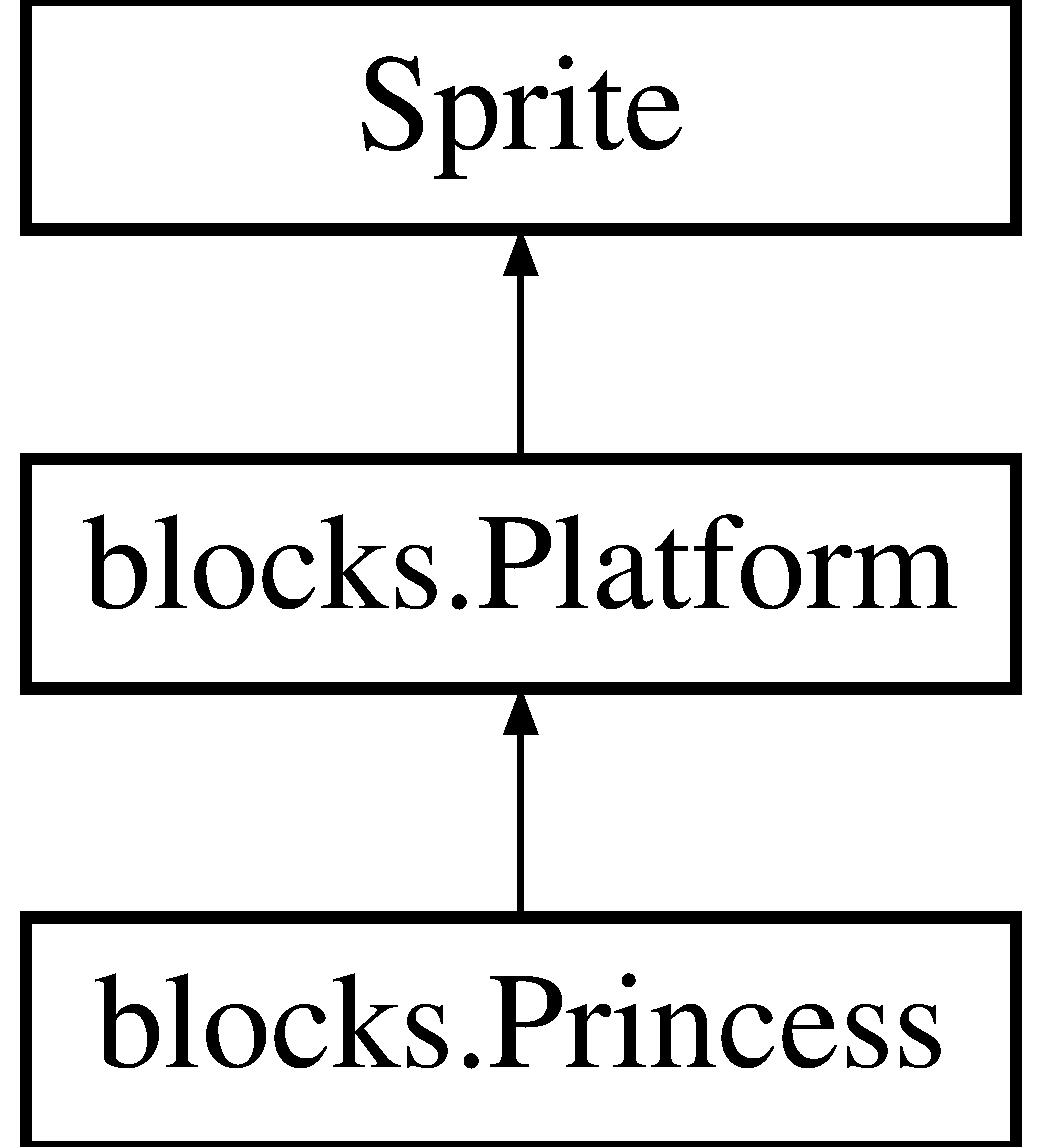
\includegraphics[height=3.000000cm]{classblocks_1_1_princess}
\end{center}
\end{figure}
\subsection*{Public Member Functions}
\begin{DoxyCompactItemize}
\item 
def \hyperlink{classblocks_1_1_princess_a7eb9ebd64a2b060dec5bf0fc69ec072f}{\+\_\+\+\_\+init\+\_\+\+\_\+} (self, x, y)
\begin{DoxyCompactList}\small\item\em The constructor. \end{DoxyCompactList}\end{DoxyCompactItemize}
\subsection*{Public Attributes}
\begin{DoxyCompactItemize}
\end{DoxyCompactItemize}


\subsection{Detailed Description}
The end of the game. 

\subsection{Constructor \& Destructor Documentation}
\index{blocks\+::\+Princess@{blocks\+::\+Princess}!\+\_\+\+\_\+init\+\_\+\+\_\+@{\+\_\+\+\_\+init\+\_\+\+\_\+}}
\index{\+\_\+\+\_\+init\+\_\+\+\_\+@{\+\_\+\+\_\+init\+\_\+\+\_\+}!blocks\+::\+Princess@{blocks\+::\+Princess}}
\subsubsection[{\texorpdfstring{\+\_\+\+\_\+init\+\_\+\+\_\+(self, x, y)}{__init__(self, x, y)}}]{\setlength{\rightskip}{0pt plus 5cm}def blocks.\+Princess.\+\_\+\+\_\+init\+\_\+\+\_\+ (
\begin{DoxyParamCaption}
\item[{}]{self, }
\item[{}]{x, }
\item[{}]{y}
\end{DoxyParamCaption}
)}\hypertarget{classblocks_1_1_princess_a7eb9ebd64a2b060dec5bf0fc69ec072f}{}\label{classblocks_1_1_princess_a7eb9ebd64a2b060dec5bf0fc69ec072f}


The constructor. 


\begin{DoxyParams}{Parameters}
{\em self} & the object pointer \\
\hline
{\em x} & the x location \\
\hline
{\em y} & the y location \\
\hline
\end{DoxyParams}


The documentation for this class was generated from the following file\+:\begin{DoxyCompactItemize}
\item 
blocks.\+py\end{DoxyCompactItemize}

\hypertarget{classpyganim_1_1_pyg_animation}{}\section{pyganim.\+Pyg\+Animation Class Reference}
\label{classpyganim_1_1_pyg_animation}\index{pyganim.\+Pyg\+Animation@{pyganim.\+Pyg\+Animation}}
Inheritance diagram for pyganim.\+Pyg\+Animation\+:\begin{figure}[H]
\begin{center}
\leavevmode
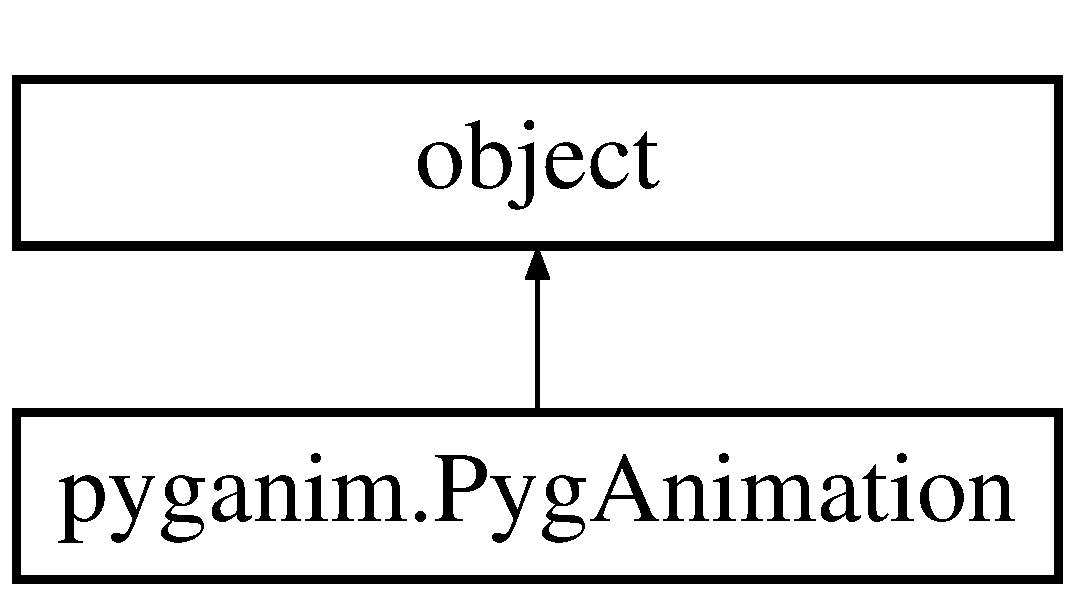
\includegraphics[height=2.000000cm]{classpyganim_1_1_pyg_animation}
\end{center}
\end{figure}
\subsection*{Public Member Functions}
\begin{DoxyCompactItemize}
\end{DoxyCompactItemize}
\subsection*{Public Attributes}
\begin{DoxyCompactItemize}
\end{DoxyCompactItemize}
\subsection*{Properties}
\begin{DoxyCompactItemize}
\end{DoxyCompactItemize}


The documentation for this class was generated from the following file\+:\begin{DoxyCompactItemize}
\item 
pyganim.\+py\end{DoxyCompactItemize}

\hypertarget{classpyganim_1_1_pyg_conductor}{}\section{pyganim.\+Pyg\+Conductor Class Reference}
\label{classpyganim_1_1_pyg_conductor}\index{pyganim.\+Pyg\+Conductor@{pyganim.\+Pyg\+Conductor}}
Inheritance diagram for pyganim.\+Pyg\+Conductor\+:\begin{figure}[H]
\begin{center}
\leavevmode
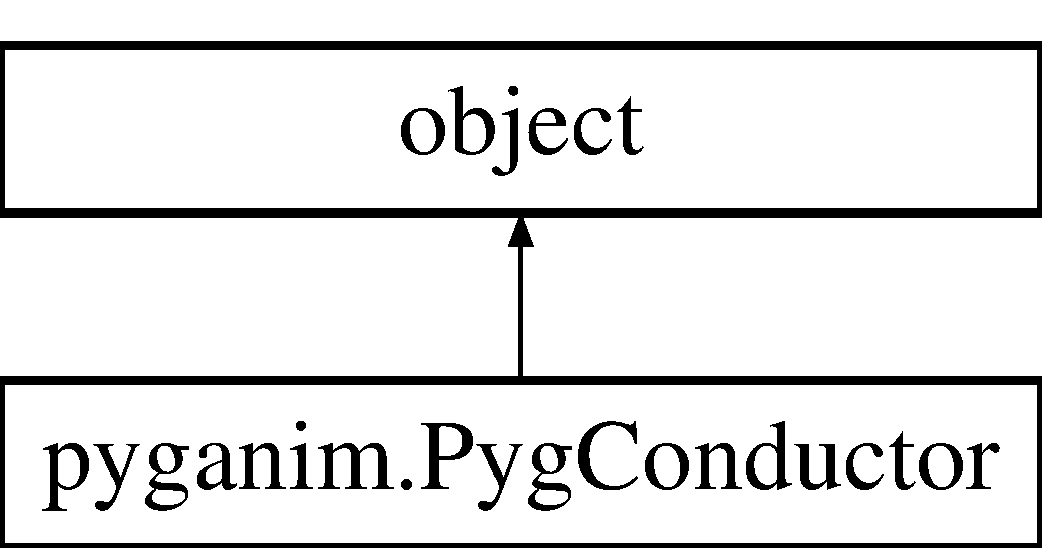
\includegraphics[height=2.000000cm]{classpyganim_1_1_pyg_conductor}
\end{center}
\end{figure}
\subsection*{Public Member Functions}
\begin{DoxyCompactItemize}
\end{DoxyCompactItemize}
\subsection*{Properties}
\begin{DoxyCompactItemize}
\end{DoxyCompactItemize}


The documentation for this class was generated from the following file\+:\begin{DoxyCompactItemize}
\item 
pyganim.\+py\end{DoxyCompactItemize}

%--- End generated contents ---

% Index
\backmatter
\newpage
\phantomsection
\clearemptydoublepage
\addcontentsline{toc}{chapter}{Index}
\printindex

\end{document}
